\documentclass{scrartcl}

\usepackage{amsmath}
\usepackage{amssymb}
\usepackage{amsthm}
\usepackage{mathtools}

%\usepackage{libertinus}

\usepackage[math-style=ISO, bold-style=ISO]{unicode-math}
%\usepackage[math-style=TeX, bold-style=TeX]{unicode-math}

\setmainfont{EB Garamond}
\setmathfont{Garamond-Math.otf}[StylisticSet={2,7,9}]
\addtokomafont{disposition}{\rmfamily}

\usepackage[english]{babel}
\usepackage{hyperref}

\usepackage{xcolor}
\hypersetup{
    colorlinks,
    linkcolor={red!50!black},
    citecolor={blue!50!black},
    urlcolor={blue!80!black}
}

\DeclareMathOperator{\eigvals}{eigvals}
\DeclareMathOperator{\diag}{diag}
\DeclareMathOperator{\abs}{abs}
\DeclareMathOperator{\CovStr}{Cov}
\DeclareMathOperator{\VarStr}{Var}
\DeclareMathOperator{\EStr}{E}
\DeclareMathOperator*{\argmax}{arg\,max}
\DeclareMathOperator*{\argmin}{arg\,min}
\DeclareMathOperator{\vecSpan}{span}
\DeclareMathOperator{\jacdet}{jacdet}

\DeclarePairedDelimiter{\norm}{\lVert}{\rVert}
\DeclarePairedDelimiterXPP{\Var}[1]{\VarStr}(){}{#1}
\DeclarePairedDelimiterXPP{\Cov}[1]{\CovStr}(){}{#1}
\DeclarePairedDelimiterXPP{\E}[1]{\EStr}(){}{#1}

\newtheorem{thm}{Theorem}
\newtheorem{cor}{Corollary}

\title{Fisher Divergence for mass matrix adaptation}
\author{Adrian Seyboldt}


\begin{document}

\maketitle

\section{Introduction}

The choice of mass matrix is known to be critical for the performance of HMC
samplers. Mass matrices are usually adapted during tuning, and convergence
speed to a good mass matrix has a big impact on the total cost of posterior
sampling as well.

todo add references to important hmc/nuts papers.

In the case of normal posterior $N(\mu, \Sigma)$ we can use the condition
number of $\Sigma$ as an estimate of how difficult it is to sample from
this posterior with an identity mass matrix.

\[
\kappa(\Sigma) = \frac{\max{\eigvals(\Sigma)}}{\min{\eigvals(\Sigma)}}
\]

If we use a mass matrix $\hat{\Sigma}^{-1}$, we can compute the
condition number by replacing the eigenvalues by the generalized eigenvalues
with respect to the inverse mass matrix $\eigvals(\Sigma, \hat\Sigma)$.

A better estimate can be found
here\footnote{\url{https://arxiv.org/pdf/1905.09813.pdf}}, but for our purposes
the simpler condition number will do fine.

Currently, most implementations (at least Stan + PyMC) use a regularized
version of the empirical covariance or its diagonal as inverse mass matrix.

\subsection{Use gradients of posterior log density}

This means however, that we do not use an additional source of information that
we have available anyway: the gradients of the posterior log density at the
positions of the draws.

Since the gradients transform covariantly, where the draws transform
contravariantly, the covariance of gradients is the inverse covariance matrix
for a Gaussian posterior. This indicates that the covariance of the gradients
gives us an estimate for $\Sigma^{-1}$, while the variance of the draws
themselves gives an estimate for $\Sigma$. If we have few draws compared to the
dimensionality of the problem, the empirical covariances therefore contain
information about the large and small eigenvalues of the true covariance of the
posterior respectively. But since both of those are important for a good mass
matrix, as can be seen from the condition number, it stands to reason that we
can use the gradient information to improve mass matrix estimates.

Estimates of the variance with only the draws are also limited by the
Cramér-Rao bound, which is no longer the case if we consider additional
information. For instance, for a 1D Gaussian posterior one draw with its
gradient is already enough to uniquely identify the posterior distribution, and
as we will see it also provides a lot of information about the posterior in the
higher dimensional case.

\subsection{Fisher Divergence}

Choosing a mass matrix is equivalent to fitting a Gaussian distribution to the
posterior, where the inverse covariance matrix of the fitted distribution is
the mass matrix.

A natural way to incorporate the gradient information into this covariance
estimation is by minimizing the Fisher divergence (see e.g.
\url{https://arxiv.org/pdf/1905.05284.pdf}) between our estimated normal
distribution with density $q$ and the actual posterior distribution with
density $p$:

\[
  F(p, q)
    = \int \lVert \nabla \log p(\theta)
      - \nabla \log q(\theta)\rVert^2 p(\theta)d\theta.
\]

It is not immediately obvious which norm we should use here. A natural choice
becomes apparent if we remember that the mass matrix as used in HMC itself
defines a norm on the tangent parameter space. I propose to use this norm,
which means that we are looking for a distribution with density $q$ who's
gradients are close to the gradients of the target distribution $p$ \emph{as
seen by the sampler}:

$$
  F(p, q)
    = \int \lVert \nabla \log p(\theta)
      - \nabla \log q(\theta)\rVert_{\hat\Sigma}^2 p(\theta)d\theta,
$$

where the norm on the tangent space is given by $\lVert x\lVert_{\hat\Sigma}^2
= x^T \hat\Sigma x$, where $\hat\Sigma$ is the covariance of our fitted
distribution $q$.

This is equivalent to finding an affine transformation $\phi(x) = Ax + \mu$
such that

\begin{align}
F(\phi)
  &= \int \lVert \nabla \log p_\phi(\theta)
	- \nabla \log N(\phi(\theta) \mid 0, 1) \rVert^2 p(\theta) d\theta \\
	&= \int \lVert \nabla \log p_\phi(\theta) + \phi(\theta) \rVert^2 p(\theta) d\theta
	%&= \int \lVert \phi^*(\nabla \log p(\theta)) + \frac{1}{2} \nabla \log \jacdet(\phi(\theta)) + \phi(\theta) \rVert^2 p(\theta)d\theta
\end{align}
is minimal, where $p_\phi(\theta) = \lvert J_\phi\rvert^{1/2} p(\phi(\theta))$
is the transformed density and $AA^T = \hat\Sigma$ corresponds to the
covariance of our fitted Gaussian distribution, or the inverse mass matrix
and $\phi^*$ is the pullback of $\phi$.

\begin{proof}
TODO
\end{proof}

This definition is now valid for arbitrary families of diffeomorphisms $\phi$.

During sampling we have $N$ draws $\theta_i$ and gradients $\nabla \log
p(\theta_i)$, so we approximate $F$ by its Monte Carlo estimate:

\[
\hat{F}(p, q)
  = \frac{1}{N} \sum_i \lVert \nabla \log p(\theta_i)
    - \nabla \log q(\theta_i)\rVert^2_\Sigma
\]

or
\[
\hat{F}(\phi)
  = \frac{1}{N} \sum_i
    \norm{\nabla \log p_\phi(\theta_i) + \phi(\theta_i)}^2
\]

\subsection{Properties of minimization problem}

\begin{thm}
If $\phi_{\mu, A} = Ax + \mu$ and $X$ with density $p$ is such that $\Cov{X}$
and $\Cov{\nabla \log(p(X))}$ exist and are positive definite, then
$F(\phi_{\mu, A})$ is minimal iff $\mu = \E{X}$ and $AA^T$ is the
geodesic mean of $\Cov{X}$ and $\Cov{\nabla \log(p(X))}^{-1}$.

Put differently, $AA^T$ is such that
\[
d(\Cov{X}, AA^T) + d(AA^T, \Cov{\nabla\log(p(X))}^{-1}),
\]
is minimal, where $d(\Sigma, \Omega) = \norm{\log(\eigvals(\Sigma, \Omega))}$
is the geodesic distance of symmetric positive definite matrices
$\Sigma$ and $\Omega$ with respect to the intrinsic metric.

$\hat{F}$ is minimal for all $A$ with $\hat{\Sigma} AA^T\hat{\Sigma} =
\hat{\Omega}$, where $\hat{\Sigma} = \Cov{X_i}$ is the empirical
covariance of the draws and $\hat{\Omega} = \Cov{\nabla \log(p(X_i))}$ is
the empirical covariance of the gradients.
\end{thm}

\begin{proof}
See appendix.
\end{proof}

So if we interpret both $\Cov{X}$ and $\Cov{\nabla \log(p(X))}^{-1}$ as
possible choices for the inverse mass matrix, minimizing $F$ leads to the mean
of those two choices. If we have more dimensions than draws, this minimum (or
mean) is not unique however, so we will need regularization of some kind in
order to find a unique mass matrix estimate.

\begin{cor}
If $\phi$ is as above and additionally $X ~ \sim N(\mu', \Sigma')$,
then the minimum of $F$ is at $\mu = \mu'$ and $\Sigma = \Sigma'$, because in
this case $\Cov{X} = \Cov{\nabla \log(p)}^{-1}$.

Let $k$ be the number of draws in $n$ dimensions and let $\hat A$ be the linear
part of the minimizer of $\hat F$. Then there exists a $k$-dimensional
subspace of $\vecSpan(X_i, \nabla\log p(X_i))$ in which $\hat A\hat A^T$
matches the true covariance $\Sigma$ exactly.
\end{cor}

This means if our posterior is a Gaussian, we get better estimates for the mass
matrix the more draws we have, and if we have more draws than dimensions our
mass matrix estimate will be perfect.

\begin{cor}
Given a space of transformation $\phi_{\mu, \sigma}(X) = \mu + \sigma \odot X$
(this corresponds to diagonal mass matrices) $F$ is minimal if $\mu =
E_p[X]$ and $\sigma^2 = \sqrt{\frac{\Var{X}}{\Var{\nabla \log(p(X))}}}$
and

\[
\sigma
  = \argmin_{\sigma} d(\Cov{X}, \diag(\sigma)^2)
    + d(\diag(\sigma)^2, \Cov{\nabla\log(p(X))}^{-1}),
\]

$\hat F$ is minimal if
\[
\sigma^2 = \sqrt{\frac{\Var{X_i}}{\Var{\nabla \log(p(X_i)}}}.
\]
\end{cor}

This last result motivates a simple modification of the status quo diagonal
mass matrix adaptation. Instead of adapting based on the marginal variance of
each parameter, we adapt based on the geometric mean of the marginal variance
and inverse marginal variance of the gradients.

In the next part of this paper we will investigate this modification in more
detail, and compare an implementation of it in nutpie with the current default
choice.

In later parts we will show how we can develop the ideas further for
sub-quadratic mass matrix adaptation that still can deal with highly correlated
posteriors.

The final part will investigate further generalizations to non-linear
transformations using neural networks.

\section{Diagonal mass matrix}

Based on the previous results we can estimate diagonal mass matrices as

\[
\hat\Sigma^{-1} = \diag\left(\sqrt{\tfrac{\Var{X_i}}{\Var{\nabla \log(p(X_i)}}}\right).
\]

We have seen that if the posterior is Gaussian with diagonal covariance,
this will recover the exact covariance matrix with only two draws.

\subsection{Gaussian posteriors}

Posterior distributions often approximate diagonal covariances, but have some
non-diagonal components. To evaluate the new proposed diagonal mass matrix
approximation for non-diagonal Gaussian distributions we model posterior
covariance matrices as coming from a distribution defined as follows (todo add
ref for Haar distribution, uniform on orthogonal matrices):

\begin{align*}
U &\sim \text{Haar}(n) \\
\log(\lambda) &\sim N(0, \sigma_\text{vals}^2) \\
\log(d) &\sim N(0, \sigma_{diag}^2) \\
\Sigma &= \diag(d)U\diag(\lambda)U^T\diag(d)
\end{align*}

We have two hyperparameters, $\sigma_\text{vals}$ and $\sigma_{diag}$. The
first controls how much correlation structure we have (if $\sigma_\text{vals} =
0$ the correlation matrix is diagonal), the second how much the marginal
variables are scaled differently. If we sample from this distribution of
covariance matrices we can apply both mass matrix adaptation methods and
compare their respective quality using the condition number from (todo add
ref). \autoref{fig_diag_condition} shows the results of this comparison, and we
can see that the Fisher divergence based adaptation is clearly superior if we
have few draws or if the matrix is dominated by the diagonal scaling. I have
not found any covariance matrices so far where the fisher divergence based
estimate was worse (I guess that doesn't exist, but I don't have a proof).

\begin{figure}
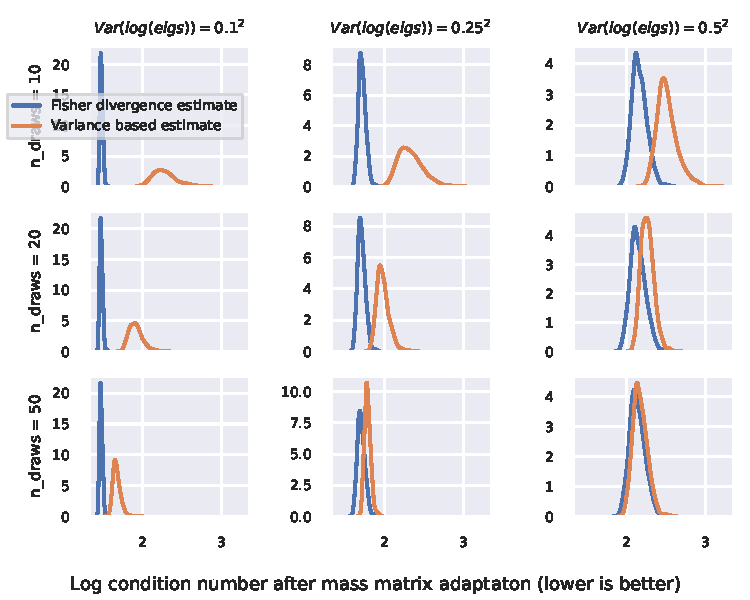
\includegraphics{figures/diag_condition_number}
\caption {Comparison of fisher divergence based diagonal mass matrix adaptation with variance based}
\label{fig_diag_condition}
\end{figure}


\begin{figure}
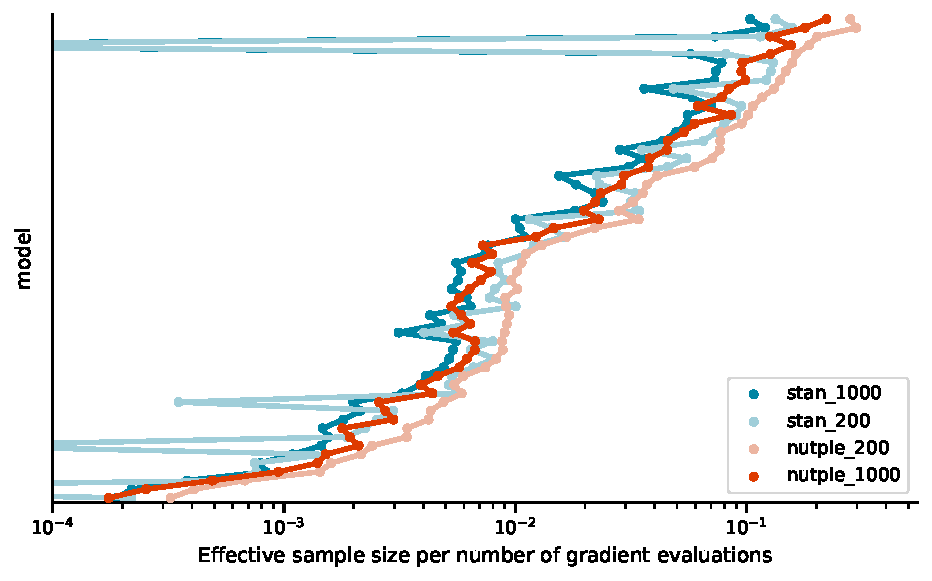
\includegraphics{figures/ess_per_grad}
\caption{
    Effective sample size for different tuning length and the fisher divergence
    based diagonal mass matrix adaptation in nutpie and the sample based
    mass matrix adaptation in Stan.
}
\label{fig_diag_condition}
\end{figure}


\subsection{Windowed algorithm implemented in nutpie}

I implemented a new mass matrix adaptation algorithm based on this new
diagonal mass matrix adaptation in \autoref{nutpie}.

In order to sample the posterior using HMC we have to solve a chicken-and-egg
problem: We need good samples from the posterior distribution in order to
figure out the mass matrix, but we need a good mass matrix estimate in order to
draw good samples. Most MCMC implementations solve this by using a warmup
phase: We start with some mass matrix estimate, use it to sample for a bit, use
those draws to improve the mass matrix and repeat. Especially at the beginning
of this phase, hmc is often quite inefficient. Stan for instance tends to start
with a number of draws with very high treesize, before it is able to find a
reasonable mass matrix. During this first phase it often uses a sizable portion
of the number of gradient evaluations it needs for warmup.

Nutpie changes this warmup method a bit: First, we can use the gradient at the
initial position to initialize the mass matrix (i.e. $M =
\diag{\abs{\text{grad}}}$), instead of initializing it using ones.

We then split the warmup period into three sections: The early, middle and late
phase. In the early phase we keep track of the variance in growing overlapping
windows, the foreground and background windows. For each new draw we update
variance estimators for draw and gradient variances with the new point, and
update the mass matrix estimate using the foreground estimates. If the
background estimators have seen a certain number of points, we use them as the
new foreground estimators, and initialize new, empty background estimators. We
continue this scheme in the middle phase, but with a larger cutoff for window
switching. In the late phase we fix the mass matrix and only update the step
size.

\subsection{Evaluation on real posterior distributions}

\autoref{posteriordb} contains a large selection of real world posterior
distributions. I ran both the Stan sampler and the nutpie sampler on each
of those posterior distributions with different number of warmup draws.
We can then measure different metrics:

\begin{itemize}
\item How many gradient evaluations did the sampler use during warmup? Note
that this is not the same as the number of warmup draws, because for each
draw we might use a different number of gradient evaluations, and depending
on current mass matrix estimate and step size those numbers might differ a lot
between sampler implementations.

\item What is the effective sample size after sampling a fixed number of draws
after warmup.

\item How many gradient evaluations were used after warmup?

\item General convergence statistics like presence of divergences and $\hat{R}$.
\end{itemize}



\section{Mass matrix with correlation structure}

Discuss some simple regularizers (is $tr(\Sigma) + tr(\Omega)$), even though
they don't seem to work all that well?

Discuss projection onto $\vecSpan(X, \nabla X)$, to reduce from $O(n^2)$ to $O(k^2)$.

Large influence of diagonal in many actual models, i.e. scale draws first?

Add epsilon to 0 eigvals trick?

Finally, the one implemented in covadapt: Matrix representation as $D(U(\Lambda
- I)U^T + I)D$, so that we can avoid strong regularization on $D$ but have
regularization on $\Lambda$, and $\Lambda$ can be much smaller than $n\times
n$, so we avoid quadratic cost: only fix a few eigenvector, eigenvalue
combinations, that cause the biggest trouble.

But we actually have to solve the minimizing problem, where we use natural
gradient decent. The parameter space is $\log(d), U, \log(\lambda) \in \mathbb{R}^n
\times \text{Stiefel}^k \times \mathbb{R}^k$. We have a natural metric, because each
point in parameter space refers to a probability distribution (information
geometry, fisher metric). We can find gradient with respect to that metric and
run manifold minimization.

The resulting algorithm: Initialize mass matrix, draw a few samples, run a few
optimization iterations and update mass matrix, repeat...

Show results from a couple of models (e.g. GP where we often have correlations).

\section{Non-linear transformations}

We need to parameterize transformations $\phi$. There is some literature on
how to do that with neural networks, I don't know that too well though.

Came up with this so far (which does seem to work quite well?):

Use a bijective neural network directly as transformation.

Activation function based on $\text{act}(x) = (1 - α)\log(1 + x) + αx$ for positive, inverse
(based on lambert W function) for negative values of $x$. This leads to nice
nonlinearity, but avoids overflows and underflows.

Each layer is $\text{act}(DA_vx + b)$, where $D$ diagonal, and $A_v = I
+ (1 - \norm{v}^{-2})vv^T$, such that all eigenvalues are one
except one with eigenvector $v$ and eigenvalue $\norm{v}^2$.

This means that each jacobian determinant is easy to compute, and we can easily
compute the objective $\hat F$.

Optimization can use SGD or maybe Levenberg–Marquardt with iterative matrix
solve using CG or so? Current implementation is a very messy notebook with some
jax code\dots

\section*{Appendix}

\begin{proof}
TODO
\iffalse
Assuming $q = N(\hat{\mu}, \hat{\Sigma})$ and differentiating by $\hat{\mu}$ and
a symmetric $\hat{\Sigma}$ gives us

\begin{align*}
\hat{\mu} &= \hat{\Sigma}\overline{\nabla \log p(\theta_i)} + \overline{\theta_i}
C &= \hat{\Sigma}P\hat{\Sigma} \\
\end{align*}

where
\begin{align*}
P &= \Cov{\nabla \log p(\theta_i), \theta_i} \\
C &= \Cov{\theta_i, \theta_i} \\
\overline{y_i} &= \frac{1}{N}\sum_i y_i
\end{align*}

TODO\dots
\fi
\end{proof}

\end{document}
